%%% File encoding: UTF-8
%% äöüÄÖÜß  <-- no German Umlauts here? Use an UTF-8 compatible editor!

%%% Magic comments for setting the correct parameters in compatible IDEs
% !TeX encoding = utf8
% !TeX program = pdflatex 
% !TeX spellcheck = de_DE
% !BIB program = biber

\documentclass[master,german]{hgbthesis}
% Permissible options in [..]: 
%   Type of work: diploma, master (default), bachelor, internship 
%   Main language: german, english (default)
%%%----------------------------------------------------------

\RequirePackage[utf8]{inputenc}		% Remove when using lualatex or xelatex entfernen!
\usepackage{graphicx}
\usepackage{svg}
\usepackage{minted}
\usepackage{listings}
\usepackage{varioref}
\usepackage{longtable}
\usepackage{tabularx}
\usepackage{parskip}
\usepackage{url}


\geometry{top=2.5cm,left=2.5cm,bottom=2.5cm,right=2.5cm}

% -----------------------------------------------------
\newenvironment{code}{\captionsetup{type=listing}}{}
% -----------------------------------------------------
% -----------------------------------------------------
\newcommand{\mysubsubsection}[1]{{\subsubsection{\textbf{#1}}}}
\newcommand{\mentionedtext}[1]{{\textit{{#1}}}}
\newcommand{\sourceDir}{./sources}
\newcommand{\sourceFontSize}{\fontsize{10pt}{11.5}}
\newcommand{\quotes}[1]{``#1''}
\newmintedfile[bashFile]{bash}{
	linenos=false, 
	frame=none, 
	breaklines=true, 
	tabsize=2,
	numbersep=5pt,
	xleftmargin=10pt,
	baselinestretch=1,
	fontsize=\sourceFontSize
}
\newmintedfile[yamlFile]{yaml}{
	linenos=false, 
	frame=none, 
	breaklines=true, 
	tabsize=2,
	numbersep=5pt,
	xleftmargin=10pt,
	baselinestretch=1,
	fontsize=\sourceFontSize
}
\newmintedfile[javaFile]{java}{
	linenos=false, 
	frame=none, 
	breaklines=true, 
	tabsize=2,
	numbersep=5pt,
	xleftmargin=10pt,
	baselinestretch=1,
	fontsize=\sourceFontSize
}
\newmintedfile[xmlFile]{xml}{
	breaklines=true, 
	tabsize=2,
	numbersep=5pt,
	xleftmargin=10pt,
	baselinestretch=1,
	autogobble=true,
	breakautoindent=false,
	fontsize=\sourceFontSize
}
\newmintinline[inlineJava]{java}{
	fontsize=\sourceFontSize
}
\newmintinline[inlineBash]{bash}{
	fontsize=\sourceFontSize
}
% -----------------------------------------------------
\graphicspath{{images/}}    % location of images and graphics
\logofile{logo}				% logo file = images/logo.pdf (use \logofile{} for no logo)

\bibliography{references.bib}  	% name of bibliography file (references.bib)

\setlength{\parindent}{0pt}
\usepackage{titlesec}

\titleformat{\section}
{\normalfont\Large\bfseries}{\thesection}{1em}{}

\renewcommand*{\labelalphaothers}{}
\DeclareLabelalphaTemplate{
	\labelelement{
		\field[final]{shorthand}
		\field{labelname}
		\field{label}
	}
	\labelelement{
		\literal{,\addhighpenspace}
	}
	\labelelement{
		\field{year}
	}
}


%%%----------------------------------------------------------
% Title page entries
%%%----------------------------------------------------------

%%% Entries for ALL types of work: --------------------------
%\title{Implementierung einer Partnerdatenbank und Evaluierung des verwendeten Technologiestack} %no camel used (and Camel)
%\author{Ing. Thomas Herzog B.Sc}
%\programname{Software Engineering}
\placeofstudy{Hagenberg}
\dateofsubmission{2020}{05}{30}	% {YYYY}{MM}{DD}

%%% Entries for Bachelor theses only: -----------------------
%\thesisnumber{XXXXXXXXXX-A}   %e.g. 1310238045-A  
% (Stud-ID, A = 1st Bachelor thesis)
%\semester{Fall Semester 2017} 	% Fall/Spring Semester YYYY
%\coursetitle{Introduction to Trivial Problems 1} 
\advisor{FH-Prof. DI Dr. Herwig Mayr}

%%% Restricted publication license instead of CC (master only):
%\cclicense

%%%----------------------------------------------------------
\begin{document}
%%%----------------------------------------------------------

%%%----------------------------------------------------------
\frontmatter							% title part (roman page numbers)
%%%----------------------------------------------------------

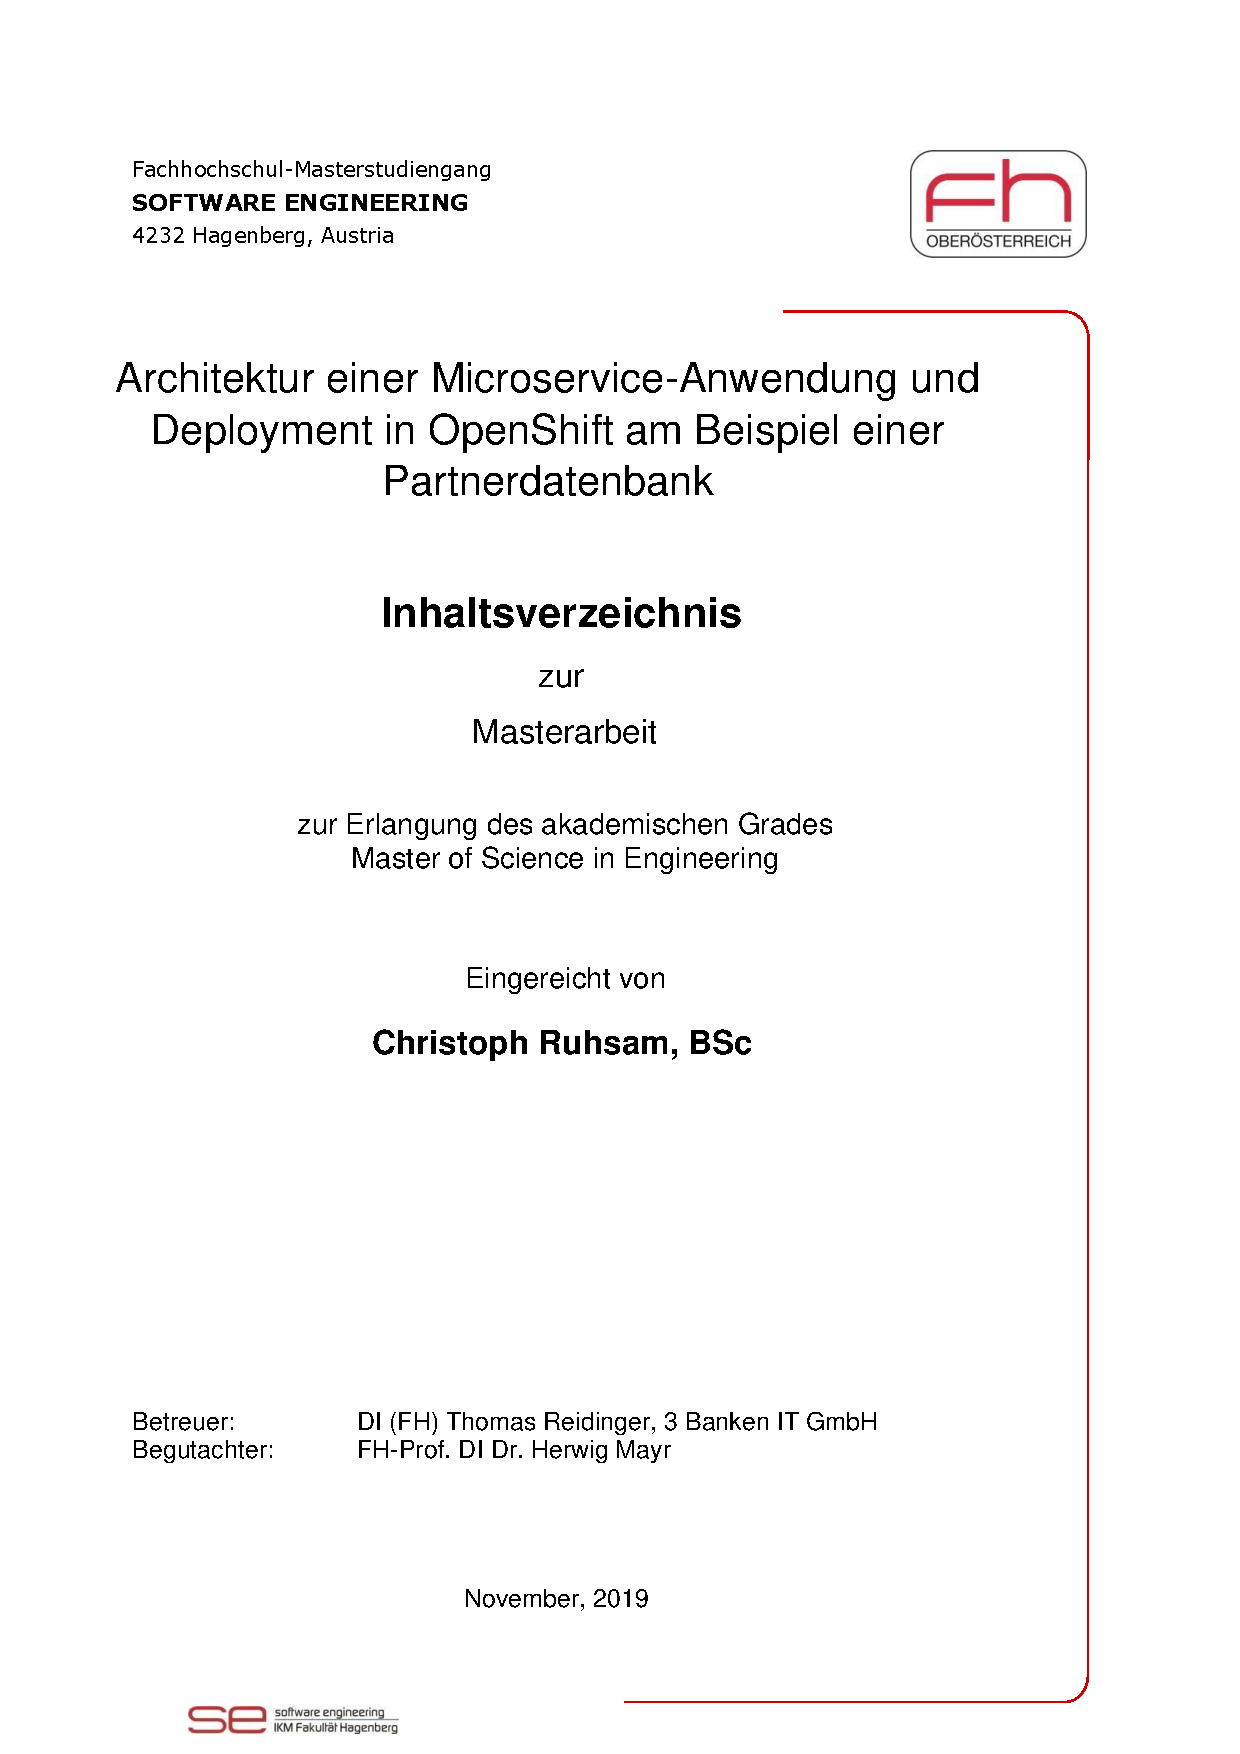
\includepdf{title.pdf}
%\maketitle
\tableofcontents

%\chapter{Preface}






 	% preface is optional
%\chapter{Abstract}
An Enterprise Service Bus (ESB) is a crucial part of an enterprise, which connects the enterprise to its partners, customers, and other branches. The appearance of containerization, cloud services, and the microservice architecture have provided new possibilities for implementing and running an ESB. But, an ESB is commonly used by large conservative enterprises, which don't adapt new technologies fast, and wait until a new technology has proven itself. Especially the cloud is something the industry denied to use for a long time, because of the fact, that the infrastructure and data are managed and maintained by external service providers. \\ 

These days, we live in the so called cloud age, whereby global enterprises like Red Hat or Amazon provide cloud services such as Platform as a Service (PaaS), which can scale with the business. Enterprises start to consider to move their ESB installations to the cloud to profit from the cloud service provided features. Moving an ESB to the cloud will be a long term process for an enterprise, because the established processes for development, running, and managing the ESB will have to change. \\

This thesis has the goal to give the reader an overview of the cloud related concepts and technologies such as, Infrastructure as Code (IaC) and Docker, which are the base for cloud services. The implemented ESB prototype,  is  available at \url{https://github.com/cchet-thesis-msc/prototype}, and shows how an ESB could be implemented on a PaaS platform. \\




%%%----------------------------------------------------------
\mainmatter          			% main part (arabic page numbers)
%%%----------------------------------------------------------

\chapter{Einleitung ... 5.5 Seiten}
\section{Motivation zur Architektur von Microservices ... 1.5 Seiten}
\section{Motivation zum Einsatz von Cloudtechnologien ... 1.5 Seiten}
\section{Zielsetzung der Implementierung der Partnerdatenbank ... 1 Seite}
\section{Ziel des Deployments der Partnerdatenbank in OpenShift ... 1 Seite}
\section{Leitfaden und Gliederung der Schrift ... 0.5 Seiten}

\chapter{Serviceorientierte Architektur und Microservices}
Das folgende Kapitel behandelt Microservices, ihre Vor- und Nachteile und die Abgrenzung zu serviceorientierten Architekturen sowie die Unterschiede zu monolithischen Architekturen.
\section{Definition und Abgrenzung}
Im Folgenden werden die Definition von Microservices und die Abgrenzung zu serviceorientierten Architekturen beschrieben.

\subsection{Definition von Microservices}
Microservices sind ein Ansatz, um große Softwarearchitekturen in kleine, konsistente, voneinander klar abgegrenzte Services zu zerlegen. Diese Services sind isoliert und kommunizieren miteinander \cite{MicroservicesForJavaDevelopers}.

Microservices werden typischerweise von kleinen Teams implementiert, gebaut und deployt. Diese kleinen Services sind so autonom, dass das Team, welches für den Service zuständig ist, die Implementierungsdetails ändern kann, ohne großen Einfluss auf das gesamte restliche System zu haben.
Jedes Team ist selbst für sein Service verantwortlich. Das Team muss für die Aufgabenstellung die richtige Technologie wählen, das Service deployen und managen und etwaige Fehler beheben.
Bei Microservice-Architekturen kann die Abgrenzung der verschiedenen Services ganz klar definiert werden. \cite{MicroservicesForJavaDevelopers} Dies hilft, um \cite{MicroservicesForJavaDevelopers}:
\begin{enumerate}
	\item \label{SOA:Abgrenzung:logik} die Logik des Services einfach zu verstehen, ohne den Kontext der gesamten Applikation kennen zu müssen,
	\item \label{SOA:Abgrenzung:bauen} den Service schnell lokal bauen und ausführen zu können,
	\item \label{SOA:Abgrenzung:technologie} die richtige Technologie für ein Problem zu nützen,
	\item \label{SOA:Abgrenzung:testen} den Service einfach und schnell testen zu können, ohne die gesamte Applikation dabei hochfahren zu müssen,
	\item \label{SOA:Abgrenzung:release} schnellere Releasezeiten zu ermöglichen,
	\item \label{SOA:Abgrenzung:skalierung} schnellere horizontale Skalierung zu ermöglichen,
	\item \label{SOA:Abgrenzung:belastbarkeit} die Belastbarkeit des Systems zu verbessern.
\end{enumerate}

Die oben angeführten Punkte werden im Folgenden näher ausgeführt \cite{MicroservicesForJavaDevelopers}:

\textbf{\ref{SOA:Abgrenzung:logik} Logik}: Jedes einzelne Microservice sollte nur einen Teil der gesamten Anwendung ausmachen. Ein Microservice deckt meist nur einen Geschäftsfall der gesamten Businesslogik ab. Dieser Geschäftsfall ist für sich einfacher zu verstehen als das gesamte System. Kommt ein neuer Entwickler in das Team, muss er sich nur in den Code des Microservice, an dem er arbeitet, einlesen und muss nicht das gesamte System verstehen.

\textbf{\ref{SOA:Abgrenzung:bauen} Bauen und Ausführen}: Muss bei einem neuen Feature die gesamte Anwendung gebaut, deployt und ausgeführt werden, ist dies sehr aufwändig und kostet sehr viel Zeit. Ein Microservice hingegen steht für sich selbst und kann einfach lokal gestartet und getestet werden. Dies erleichtert dem Entwickler die Arbeit und spart Zeit.

\textbf{\ref{SOA:Abgrenzung:technologie} Technologie}: Meist werden für bestimmte Geschäftsfälle verschiedene Technologien benötigt. Ist die gesamte Businesslogik in einem Monolithen abgebildet, kann lediglich eine Technologie eingesetzt werden. Ist aber beispielsweise für einen bestimmten Geschäftsfall Machine Learning nötig, ist eventuell Java die falsche Lösung und man setzt lieber auf Python.
Microservices sind unabhängig voneinander und kommunizieren meist durch REST oder SOAP (siehe dazu Abschnitt \ref{subsec: AbgrenzungServiceorientierte}) miteinander. Dadurch kann in jedem Service die gewünschte Technologie eingesetzt werden.

\textbf{\ref{SOA:Abgrenzung:testen} Testen}: Ähnlich zu \ref{SOA:Abgrenzung:bauen}, wo das Bauen und Ausführen eines Microservice beschrieben wird, kann ein Service auch unabhängig vom gesamten System getestet werden.

\textbf{\ref{SOA:Abgrenzung:release} Releasezeiten}: Heutzutage müssen neue Features schnell ausgeliefert werden, ansonsten ist womöglich der Konkurrent schneller und man verliert Kunden. Muss bei einem neuen Release das gesamte System neu deployt werden, sind damit verschiedenste Risiken verbunden. Wird z.B. ein fehlerhafter Code deployt, stürzt der gesamte Monolith ab. Bei Microservices ist in dieser Zeit lediglich das neu deployte Service nicht verfügbar.

\textbf{\ref{SOA:Abgrenzung:skalierung} Skalierung}: Hat man ein monolithisches System und möchte einen neuen Geschäftsfall implementieren, muss dieser in das bestehende System eingeflochten werden, was dazu führen kann, dass ein bestehender Code nicht mehr so funktioniert wie gewollt.
Bei einer Microservice-Architektur wird ein neues Service für diesen Geschäftsfall angelegt und bestehender Code nicht oder kaum für Aufrufe des neuen Service geändert.

\textbf{\ref{SOA:Abgrenzung:belastbarkeit} Belastbarkeit}: Fällt ein Service aus, heißt das nicht, dass das gesamte System nicht mehr verfügbar ist. Teile des Systems können meist ohne Probleme weiterverwendet werden.



\subsection{Abgrenzung serviceorientierter Architekturen und Microservices}
\label{subsec: AbgrenzungServiceorientierte}
Microservices und serviceorientierte Architekturen gehören beide zu den service-basierten Architekturen. Das heißt, dass beide Architekturen einen großen Schwerpunkt auf Services als primäre Architekturkomponenten legen. Obwohl Microservices und serviceorientierte Architekturen sehr unterschiedliche Muster aufweisen, haben sie auch viele Gemeinsamkeiten \cite{MicroservicesVSSOA}.

Alle serviceorientierten Architekturen sind verteilte Architekturen. Die Servicekomponenten werden über Remote-Protokolle, wie beispielsweise Representational State Transfer (REST), Simple Object Access Protocol (SOAP) oder Java Message Service (JMS) angesprochen.
Beide bieten viele Vorteile im Vergleich zu monolithischen und schichten-basierten Architekturen. Sie bieten höhere Skalierbarkeit, losere Kopplung zwischen den Services und bessere Kontrolle über Entwicklung, Tests und Deployment. Komponenten in einer verteilten Anwendung tendieren mehr dazu, in sich geschlossen zu sein und bieten daher besseres Änderungsmanagement und einfachere Wartung, was zu mehr Flexibilität und zu robusteren Anwendungen führt.
Diese Architekturen führen auch zu loser gekoppelten und modulareren Anwendungen. 
Modularität bedeutet das Kapseln einzelner Teile der Anwendung in abgeschlossene Services, die dadurch individuell designt, entwickelt, getestet und deployt werden können, ohne großen Einfluss auf andere Services zu nehmen \cite{MicroservicesVSSOA}.

Sowohl bei Microservices als auch bei serviceorientierten Architekturen müssen \textit{Service Contracts} vereinbart werden. Service Contracts werden zwischen einem Service und einem Servicekonsumenten (Client) vereinbart. Dadurch wird das Format der eingehenden und ausgehenden Daten spezifiziert (z.B. XML, JavaScript Object Notation [JSON], Java Object, etc.) \cite{MicroservicesVSSOA}. 

Microservice-Teams bestehen meist aus maximal sieben Personen. Das Team muss die Entwicklung, das Deployment und den Betrieb des Service alleine bewältigen. Je größer das Team, desto höher ist der Kommunikationsaufwand. Jedes Teammitglied sollte die gesamte Codebasis überblicken und warten können. Zu große Teams sind meist ein Indikator dafür, dass das Service aufgesplittet werden sollte \cite{MicroservicesVSSOA}.

Serviceorientierte Architekturen sind eher für große, komplexe Enterprise-Systeme geeignet, die eine Interaktion mit vielen heterogenen Applikationen und Services benötigen. Für Anwendungen, die viele Komponenten benötigen und von mehreren Services geteilt werden, sind serviceorientierte Architekturen passend.
Für Applikationen mit einem wohldefinierten Arbeitsablauf und wenig gemeinsam geteilten Komponenten, wie z.B. Security-Komponenten, sind Microservice-Architekturen sinnvoll.
Microservice-Architekturen sind besser geeignet für kleine, wohl definierte, web-basierte Systeme, als für groß skalierbare Enterprise-Systeme. Die fehlende Middleware ist ein Faktor, weshalb Microservice-Architekturen nicht oder schlecht für komplexe Businessanwendungen geeignet sind. Microservices sollten dort eingesetzt werden, wo sich die Businesslogik auf kleine, abstrahierte Geschäftsfälle herunterbrechen lässt \cite{MicroservicesVSSOA}.

Microservices und serviceorientierte Architekturen sind auch bezüglich Teilen von Komponenten sehr unterschiedlich. Serviceorientierte Architekturen basieren auf dem Prinzip \textit{share-as-much-as-possible}, wohingegen Microservices auf dem Prinzip \textit{share-as-little-as-possible} basieren.
Angenommen, ein großes Warenhaus benötigt zum Verwalten der Einkäufe und Verkäufe jeweils ein \textit{Bestellservice}. Bei serviceorientierten Architekturen, wie in Abbildung \ref{fig:SOA_Bestellservice} zu sehen, würde man dazu das Bestellservice einmal implementieren und die Einkaufs- und Verkaufskomponente teilen sich dieses Service. Das Bestell-Service selbst muss in diesem Fall wissen, welche Aktionen es bei den verschiedenen Anfragen ausführen muss.
Obwohl das \textit{share-as-much-as-possible}-Prinzip das Problem der Codeduplizierung löst, ist damit eine enge Kopplung von Businesskomponenten verbunden und erhöht das Risiko bei Änderungen. Angenommen, man ändert den Code im Business-Service, ist diese Änderung schwer zu testen, da das Service global verfügbar ist und je nach Aufruf andere Aktionen auslöst \cite{MicroservicesVSSOA}.

\begin{figure}[H]
	\begin{center}
		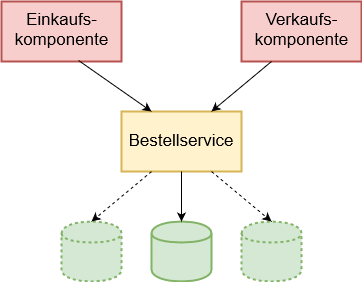
\includegraphics[scale=0.80]{SOA_Bestellservice.png}
		\caption[Serviceorientierte Architektur - Bestellservice]{Serviceorientierte Architektur - Bestellservice \cite{MicroservicesVSSOA}}
		\label{fig:SOA_Bestellservice}
	\end{center}
\end{figure}

Microservices basieren auf dem Konzept \textit{share-as-little-as-possible} und verstärken dadurch das Domain-driven Designkonzept \textit{Bounded Context}. Microservices sind lose gekoppelt und agieren daher als einzelne geschlossene Einheit mit wenig Abhängigkeiten. Es gibt lediglich ein wohldefiniertes Interface und wohldefinierte Vereinbarungen nach außen. 
Realistischerweise wird es immer gemeinsam geteilte Services geben, auch in Microservice-Architekturen, z.B. Sicherheits- oder Infrastrukturservices. Serviceorientierte Architekturen maximieren das Teilen von Komponenten, wohingegen Microservice-Architekturen das Teilen durch den klar definierten Bounded Context minimieren \cite{MicroservicesVSSOA}.

Es gibt viele Vorteile, die das Verstärken des Bounded Context bringt. Die Wartung der Services wird wegen der geringeren Abhängigkeiten weitaus einfacher. Dies erleichtert auch das Ändern und Weiterentwickeln des Services. Auch das Deployment gestaltet sich dadurch um einiges einfacher, da weniger Code zu deployen ist und es weniger Risiken gibt, andere Bereiche des gesamten Systems zu brechen. Dies fördert auch die Robustheit des gesamten Systems \cite{MicroservicesVSSOA}.


\section{Vergleich mit monolithischer Architektur}
Microservices und Monolithen sind sehr unterschiedliche Designstrategien, um eine Anwendung zu entwickeln. Beide Strategien haben ihre Vor- und Nachteile. Die Strategie sollte deshalb mit Bedacht gewählt werden. Die monolithische Architektur ist derzeit noch der Standardweg,  eine Applikation zu entwickeln \cite{FowlerDSM}.

Im Folgenden werden die wichtigsten Unterschiede von monolithischen und von Microservice-Architekturen beschrieben \cite{MonolithVSMicroservices}.

\subsection{Wartung}
Microservices sind viel einfacher zu warten, da sich die Komplexität eines Services in Grenzen hält. Microservices sind modulare und unabhängige Services. Neue Entwickler können sich in die Codebasis schneller einlesen und schneller neue Features implementieren als bei monolithischen Architekturen.

Ein Monolith besteht aus einer Codebasis, in der alle Geschäftsfälle abgedeckt sind. Wird ein neues Feature hinzugefügt, wird es dabei in die bestehende Codebasis eingewebt. 
Dies erhöht die Komplexität des Codes und erschwert die Entwicklung und Wartung.
Neue Entwickler müssen sich in die gesamte Codebasis und in den gesamten Workflow einlesen, um neue Features entwickeln zu können.

\subsection{Deployment}
Ein kontinuierliches Deployment gestaltet sich bei Monolithen sehr schwierig, da der Monolith immer größer und komplexer wird. Zudem muss immer der gesamte Monolith deployt werden, auch wenn lediglich wenig Codestücke geändert wurden. Dies ist natürlich sehr zeitaufwändig, aber auch gefährlich. Wird ein fehlerhafter Code deployt, bringt dieser den gesamten Monolith zum Stillstand.

Bei Microservices hingegen wird die Codebasis in kleine, überschaubare Services unterteilt, die einzeln und jederzeit schnell deployt werden können. Wird bei Microservice-Architekturen ein fehlerhafter Code deployt, ist es möglich, dass andere Teile des gesamten Systems noch ohne Probleme laufen.

\subsection{Tests}
Auch beim Testen eines Monolithen werden die große Codebasis und die vielen verschiedenen Anwendungsfälle zum Problem. Das Testen aller Szenarien bei einer derart großen Codebasis wird dabei schnell unübersichtlich.

Bei Microservices kann durch den Bounded Context jede Komponente individuell getestet werden. Dies erleichtert das Testen eines jeden Services ungemein und verringert zusätzlich die Fehleranfälligkeit eines Systems.

\subsection{Startup-Zeit}
Bei monolithischen Architekturen wird der gesamte Monolith hochgefahren. Je komplexer und größer dieser wird, desto mehr steigt die Startzeit.

Die Startzeit bei Microservices ist viel schneller, da jedes Service einzeln hochgefahren werden kann. Werden alle Services gemeinsam gestartet, bringt dies bezüglich der Startzeit wieder wenig.

\subsection{Technologie}
Ein Monolith wird in einer Programmiersprache entwickelt und greift meist nur auf eine Datenbank zu. Neue Technologien können nicht bzw. nur sehr umständlich hinzugefügt werden. Die Einarbeitungszeit gestaltet sich jedoch bezüglich Technologie einfacher, da nur eine Sprache zum Einsatz kommt und neue Entwickler nur diese beherrschen müssen.

Mit Microservices können Entwickler die Technologie jedes Services selbst wählen. Da Microservices so klein und überschaubar sind, können diese schnell ersetzt werden und es kann dadurch immer die aktuellste Version oder Technologie verwendet werden.

\subsection{Skalierbarkeit}
Microservices können einfach skaliert werden. Platform-as-a-Service-Plattformen, wie OpenShift, bieten eine einfache Möglichkeit, Services je nach Bedarf hoch- und runterskalieren zu können.

Einen komplexen Monolithen zu skalieren gestaltet sich sehr schwierig. Zum Beispiel wird ein kontinuierliches Deployment mit vielen Entwicklern und einer sehr großen Codebasis sehr kompliziert.


\section{Charakteristiken}
Im Folgenden werden die wichtigsten Charakteristiken von Microservices beschrieben, die auch für serviceorientierte Architekturen gelten \cite{SpringMicroservices}.

\subsection{Service-Vereinbarung}
Microservices werden durch wohldefinierte Service-Vereinbarungen beschrieben. Zum Datenaustausch kann z.B. REST oder SOAP verwendet werden. Als Markup-Sprache kann JSON, XML oder auch YAML eingesetzt werden. In der Welt der Microservices wird meist die Kombination von REST und JSON eingesetzt. Es gibt aber mehrere Möglichkeiten zur Definition von Service-Kontrakten. JSON Schema, WADL, Swagger und RAML sind nur ein paar wenige Beispiele.

\subsection{Lose Kopplung}
Microservices sind unabhängig und lose gekoppelt. Meist akzeptieren Microservices ein Event als Input und reagieren darauf erneut mit einem Event. Nachrichten, HTTP und REST werden häufig zur Interaktion zwischen den einzelnen Services eingesetzt. Nachrichten-basierte Endpunkte bieten dabei ein höheres Level an Entkopplung.

\subsection{Service-Abstraktion}
Service-Abstraktion bei Microservices ist nicht nur die abstrahierte Realisierung des Service, sondern bietet auch eine komplette Abstraktion von allen Bibliotheken und Umgebungsdetails.

\subsection{Wiederverwendung}
Microservices sind wiederverwendbare Business-Services. Sie werden von mobilen Geräten, Desktop-Anwendungen und auch anderen Microservices verwendet.

\subsection{Zustandslosigkeit}
Wohl-designte Microservices sind zustandslos und teilen sich nichts. Wird ein gemeinsamer Zustand in verschiedenen Services benötigt, wird dieser meist in einer Datenbank abgebildet.

\subsection{Interoperabilität}
Services sind durch Standardprotokolle und Nachrichtenaustausch-Standards interoperabel. Nachrichtenaustausch, HTTP und REST werden zum Nachrichtentransport verwendet. Eine Kombination aus REST und JSON ist die populärste Methode zum Entwickeln von interoperablen Services. Wird weitere Optimierung benötigt, kommen auch andere Protokolle, wie RabbitMQ, Avro, Zero MQ oder Protocol Buffers zum Einsatz. Der Einsatz dieser Protokolle kann dabei aber auch die Interoperabilität der Services einschränken.

\subsection{Zusammensetzung}
Microservices sind zusammensetzbar. Dies wird durch Service-Orchestrierung und Service-Choreografie erreicht. Service-Orchestrierung und Service-Choreografie sind zwei Designvarianten von Microservices. Auf diese wird im nächsten Abschnitt näher eingegangen.

\section{Designvarianten}
Im Folgenden werden die beiden Varianten \textit{Service Orchestrierung} und \textit{Service Choreografie} zum Design von Microservices vorgestellt.

\subsection{Service-Orchestrierung}
Bei der Service-Orchestrierung gibt es ein zentrales Kompositionsservice, dass das entsprechende Microservice aufruft und von diesem die Antwort erwartet. Diese Nachrichten können mittels HTTP oder Socketaufrufen durchgeführt werden. Wichtig hier ist, dass diese Aufrufe sowohl synchron als auch asynchron durchgeführt werden können. Das aufgerufene Microservice muss also nicht sofort antworten, sondern kann auch später mit der Antwort ein Event im Kompositionsservice auslösen.
In diesem Muster reden die Microservices nicht miteinander, sondern nur mit dem Kompositionsservice. Dabei muss jedoch nicht für jedes Microservice dasselbe Protokoll verwendet werden, z.B. kann das Kompositionsservice mit Service A über HTTP und mit Service B über das XML/RPC-Protokoll kommunizieren \cite{PracticalMicroservices}.

Wie in Abbildung \ref{fig:SOA_Orchestrierung} zu sehen, wird dabei das Kompositionsservice zur zentralen Autorität. Hier beginnt auch die gesamte Logik, was schlechtes Design für Microservices bedeutet. Die gesamte Logik im Kompositionsservice zu haben führt zu einer Fülle von Abhängigkeiten zwischen den Services. Z.B. kann die Logik sein, dass, wenn Service A antwortet, Service B danach aufgerufen werden muss. Dies führt zu Abhängigkeiten zwischen Service A und Service B \cite{PracticalMicroservices}.

Da das Kompositionsservice der zentrale Punkt der Anwendung ist, ist dieser auch die Schwachstelle. Dieses Service muss verfügbar sein, ansonsten steht die gesamte Anwendung still. Das Kompositionsservice ist der \textit{Single-Point-of-Failure} in dieser Architektur. Dies kann aber durch Tools und Cloud-basierte Lösungen, wie Skalierung oder Clustering, gelöst werden. Zusätzlich ist das Orchestrierungsmuster schwer zu implementieren. Hat man einen Entscheidungspunkt, wird es schwer, dem verteilten Design zu folgen \cite{PracticalMicroservices}.

\begin{figure}[H]
	\begin{center}
		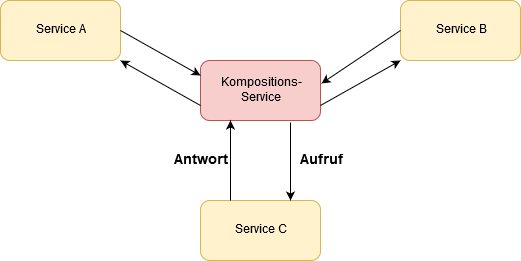
\includegraphics[scale=0.8]{SOA_Orchestration.png}
		\caption[Designvarianten - Service-Orchestrierung]{Varianten - Service-Orchestrierung \cite{PracticalMicroservices}}
		\label{fig:SOA_Orchestrierung}
	\end{center}
\end{figure}

\subsection{Service-Choreografie}
Anders als bei der Service-Orchestrierung ist bei der Service-Choreographie jedes Service in Koordination mit den anderen Services auf einen bestimmten Anwendungsfall zugeschnitten.
Service Orchestrierung repräsentiert die Kontrolle von einem einzelnen Standpunkt aus. Bei der Choreografie wird jedes Service in die Interaktion mit eingebunden \cite{PracticalMicroservices}. 

Wie in Abbildung \ref{fig:SOA_Choreographie} zu sehen, redet bei der Service Choreografie jedes Service nach Abschluss des Tasks mit einem anderen Service, um die nächste Aufgabe zu triggern. Dies kann in den Mustern \textit{one-to-one}, \textit{one-to-many} oder \textit{many-to-many} geschehen. Dies kann ebenfalls synchron oder asynchron durchgeführt werden. Idealerweise gibt es ein globales Protokoll, über das die Services miteinander kommunizieren. Meistens werden diese Aufrufe asynchron durchgeführt. Da es kein zentrales Service gibt, löst jedes Service ein Event nach Abschluss seines Tasks aus. Dies macht die Services unabhängig voneinander und fördert die lose Kopplung. Andere Services registrieren sich auf dieses Event und reagieren darauf, wenn es ausgelöst wird \cite{PracticalMicroservices}. 

Durch nachrichtenorientierte Kommunikation kann das Choreografiemuster sehr nützlich werden. Zwischen den Services wird eine Nachrichtenschlange implementiert. Dadurch wird das Loslösen, Hinzufügen und Entfernen von Services sehr einfach gelöst. Auch die ganze Reihe an Abhängigkeiten, die oft bei Choreografiemustern entstehen, wird dadurch gelöst. Service-Choreografie erhöht die Komplexität eines Systems. Jedes Service erzeugt und verarbeitet Nachrichten zur Laufzeit. Dadurch kann der exakte Stand einer Transaktion nicht herausgefunden werden \cite{PracticalMicroservices}.

\begin{figure}[H]
	\begin{center}
		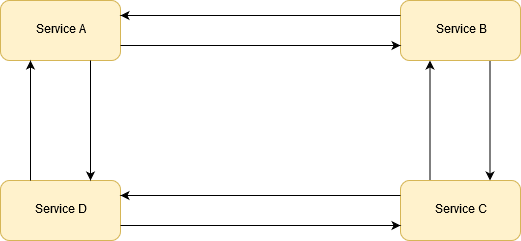
\includegraphics[scale=0.8]{SOA_Choreographie.png}
		\caption[Designvarianten - Service-Choreografie]{Varianten - Service-Choreografie \cite{PracticalMicroservices}}
		\label{fig:SOA_Choreographie}
	\end{center}
\end{figure}

\section{Vor- und Nachteile von Microservices}
Im folgenden Abschnitt werden die Vor- und Nachteile von Microservices behandelt.

\subsection{Vorteile von Microservices}
\subsubsection{Technologieunabhängigkeit}
Microservices werden als eigenständige Einheit betrachtet. Dadurch können die einzelnen Services verschiedene Technologien verwenden. Greift ein Service auf eine Datenbank zu und ein anderes Service führt Shell-Skripte aus, beeinflussen sich die beiden Services nicht und können jederzeit ausgetauscht werden, ohne Einfluss auf andere Services zu nehmen. Performanz ist in diesem Zusammenhang ebenfalls sehr wichtig. Wird eine Technologie zu langsam, kann sie ohne Probleme durch eine neue ersetzt werden \cite{Newman2015}.

\subsubsection{Skalierung}
Wie erwähnt, muss bei Monolithen die gesamte Software als Ganzes deployt und skaliert werden. Dies bedeutet viel Overhead. Bei Microservices können einzelne Teile hoch- und runterskaliert werden. Cloud-basierte Technologien, wie z.B. OpenShift, bieten diese Möglichkeit an. Es kann aber auch ein Microservice auf einer besseren Hardware laufen. Die anderen Services bleiben auf der billigeren Hardware. Monolithen müssten als Ganzes auf der besseren Hardware laufen. Dies verringert die Kosten der Skalierung bei Microservices drastisch \cite{Newman2015}.

\subsubsection{Austauschbarkeit}
Bei Microservices ist es sehr einfach, den bestehenden Code zu ändern oder auszutauschen. Da diese unabhängig sind, sind keine anderen Teile des Systems betroffen. Bei Monolithen stellt die Austauschbarkeit oft ein großes Risiko dar. Der Code ist oft sehr verwoben und kleine Änderungen haben große Auswirkungen \cite{Newman2015}.

\subsubsection{Entwicklerteam}
Entwickler greifen bei monolithischen Architekturen oft auf dieselben Teile des Codes zu. Bei Versionierungsprogrammen, wie Git oder Subversion, führt dies oft zu Konflikten.
Microservices können getrennt voneinander bearbeitet und der Code ohne Probleme zusammengefügt werden \cite{Newman2015}.


\subsection{Nachteile von Microservices}
\subsubsection{Hohe Latenzzeiten}
Microservices reden über das Netzwerk miteinander. Dieser Kommunikationsweg ist natürlich viel langsamer, als wenn diese in derselben JVM miteinander reden würden. Dies führt zu hohen Latenzzeiten. Diese müssen bei der Architektur von Microservices berücksichtigt werden \cite{Newman2015}.

\subsubsection{Wiederverwendbarkeit von Code}
Microservices sind unabhängige und eigenständige Einheiten. Sie haben im besten Fall keine Abhängigkeiten zueinander. Dadurch verringert sich die Wiederverwendbarkeit von Code. Dies führt auch zu einer Codeverdopplung. Wird dasselbe Codestück in zwei verschiedenen Services benötigt, muss es in beiden vorhanden sein \cite{Newman2015}.

\subsubsection{Deployment}
Jedes Service muss einzeln deployt werden. Dazu wird ein eigener Deployment-Prozess pro Service benötigt. Dies bedeutet Aufwand für die Entwickler und es muss eine eigene Infrastruktur geschaffen werden, was zusätzlich Kosten generiert \cite{Newman2015}.




\chapter{Containerisierung mit Docker ... 6 Seiten}
\section{Docker ... 4 Seiten}
\section{Notwendigkeit von Containerisierung ... 2 Seiten}


\chapter{OpenShift ... 10.5 Seiten}
\section{Beschreibung von OpenShift ... 2 Seiten}
\section{Komponenten von Kubernetes ... 3.5 Seiten}
\section{Die OpenShift-Umgebung ... 3 Seiten}
\section{Fabric8 ... 2 Seiten}

\chapter{Partnerdatenbank ... 14.5 Seiten}
\section{Grundaufbau und Zweck der Partnerdatenbank ... 2.5 Seiten}
\section{Backend-Beschreibung ... 4 Seiten}
\section{Beschreibung der einzelnen Services ... 4 Seiten}
\section{Frontend-Beschreibung ... 4 Seiten}

\chapter{Design der Partnerdatenbank ... 11 Seiten}
\section{Microservice-Architektur ... 3 Seiten}
\section{Beschreibung der verwendeten Microservice-Technologien ... 6 Seiten}
\section{Design in OpenShift .. 2 Seiten}


\chapter{Implementierung der Partnerdatenbank ... 17 Seiten}
\section{Microservice-Architektur ... 2 Seiten}
\section{Automatisierte Test-, Build- und Deployment-Pipelines mit Jenkins ... 3 Seiten}
\section{Fehlerbehandlung mit Microprofile ... 2 Seiten}
\section{REST-Schnittstellenbeschreibung mit Swagger ... 2 Seiten}
\section{Tracing mit Jaeger ... 1 Seite}
\section{Einsatz von Docker zur Containerisierung der Anwendung ... 1 Seite}
\section{Konfiguration und Deployment-Deskriptoren von OpenShift ... 4 Seiten}
\section{Deployment in OpenShift mit Fabric8 ... 2 Seiten}


\chapter{Evaluierung der Anwendung ... 7 Seiten}
\section{Evaluierung des Frontends ... 1.5 Seiten}
\section{Whitebox-Tests ... 2 Seiten}
\section{Blackbox-Tests ... 1.5 Seiten}
\section{Architekturevaluierung ... 2 Seiten}

\chapter{Zusammenfassung ... 2-3 Seiten}
\section{Resümee}
\section{Ausblick}


\MakeBibliography 

%%%----------------------------------------------------------
\end{document}
%%%----------------------------------------------------------